\documentclass[11pt,a4paper]{article}
\usepackage[margin=24mm]{geometry}
\usepackage[T1]{fontenc}
\usepackage{lmodern}
\usepackage{enumitem}
\usepackage{tikz}
\usetikzlibrary{positioning,arrows.meta}
\newcommand{\code}[1]{\texttt{#1}}
\title{Semantic reads in \code{hymeko\_query}: bases, is-a and field provenance}
\date{Created 2026-09-30 21:05 CEST\quad Estimate: about 1--1.5\,h}
\begin{document}
\maketitle

\paragraph{Decision.} On 2026-09-30 the user decided DS0 of core
\code{docs/plans/2026-09-30-core-after-extraction}: ``Ds0 $\to$ query''. Borrowed semantic queries
over the canonical IR belong to \code{hymeko\_query}, not Core. Core keeps the IR and its
identity. This moves the reduced S1/S2 of that plan here, and no Core edit or approval slug is
needed.

\paragraph{Evidence.}
\begin{itemize}[nosep]
\item Effective fields already live here: \code{fields.rs}, \code{effective\_child} and
  \code{effective\_value}. Geometry and webxr read them.
\item The is-a walk is written again at least eleven times across repositories. In this
  repository alone:
  \begin{itemize}[nosep]
  \item \code{engine.rs} \code{check\_inheritance}: depth 8, not reflexive;
  \item \code{predicate\_expr.rs} and \code{rewrite/template.rs}: by name, depth 16;
  \item webxr \code{isa\_transitive}: reflexive, depth 1024, a cycle reads as ``not a''.
  \end{itemize}
\item webxr's own-slot rule (\code{query.rs} \code{own}) is crate-private. HIVE and robotics
  check only that a slot is a leaf.
\end{itemize}

\paragraph{API (additive).} In a new \code{hymeko\_query/src/bases.rs}:
\begin{itemize}[nosep]
\item \code{BasePolicy::\{All, Tagged(SymId)\}} says which base relations count. A tagged base
  carries the tag symbol on its reference annotation, as \code{<isa>} does. The tag is a symbol, not
  a string, so the walk needs only the IR: webxr's validators hold no name table.
\item \code{bases(ir, decl, policy)}: the direct bases, in authored order. \code{QueryEngine}
  forwards to the free functions.
\item \code{is\_a(ir, decl, kind, policy) -> Result<bool, BaseError>}:
  \begin{itemize}[nosep]
  \item reflexive, and without a depth limit;
  \item a diamond gives one answer; the full walk visits a shared base once, and the shallow walk
    below may revisit it within its visit bound;
  \item a cycle on the walk is \code{BaseError::Cycle}, and a base outside the declaration table is
    \code{BaseError::Dangling}.
  \end{itemize}
\end{itemize}
In \code{fields.rs}:
\begin{itemize}[nosep]
\item \code{FieldBinding \{ declaration, provider \}} and \code{effective\_binding(decl, key)}.
  \code{effective\_child} becomes a thin reader over it, so the lookup rule has one
  implementation.
\item \code{own\_child(decl, key)}: the declaration's own child only, the rule a writer uses for a
  slot.
\end{itemize}

\paragraph{This slice migrates.}
\begin{itemize}[nosep]
\item webxr \code{isa\_transitive} and \code{each\_base} use \code{is\_a(..., All)}. A cycle
  still reads as ``not a'', which is today's result once the budget runs out.
\item webxr \code{own} uses \code{own\_child}.
\item A diamond fixture (S4) records the current depth-first, authored-order rule for
  \code{effective\_binding}.
\end{itemize}

\paragraph{Not in this slice.}
\begin{itemize}[nosep]
\item Query's own walks: \code{InheritsFromId} (depth 8), \code{predicate\_expr} and
  \code{template}. They change behaviour and wait for DS1/DS2.
\item Geometry, dynamics, optimize, network, \code{hymeko\_wasm} and the C port.
\item Graph (\code{hymeko\_pgraph} \code{IsaWalk}) keeps its own \code{<isa>} walk.
  Transformation depends on graph, so graph cannot depend on this crate without a repository
  cycle.
\end{itemize}

\paragraph{Open decisions.}
\begin{itemize}[nosep]
\item DS1: the policy each consumer uses. The code is split: graph and network count only
  \code{<isa>}, query and webxr count every base.
\item DS2: keep depth-first authored order, or C3, for effective fields. The S4 fixture pins the
  current rule until then.
\end{itemize}

\paragraph{Implementation record (2026-09-30).}
\begin{itemize}[nosep]
\item \code{is\_a} first tries an allocation-free walk, with its path on the call stack, up to depth 64
  and 512 visits. Beyond that it falls back to the walk that remembers finished declarations. A test
  checks that both give the same answer for every pair of declarations and both policies, cyclic IR
  included; another covers a 100-deep chain and a 12-diamond ladder.
\item webxr validation bench (release, 100k entities): 34--36\,ms before and 50\,ms after.
  Parse and lowering take about 2\,s. The first cut allocated on every call and took 212\,ms; the
  shallow walk removed most of that. The rest pays for the new dangling-base check.
\item Tests:
  \begin{itemize}[nosep]
  \item \code{hymeko\_query}: 34 unit and 220 integration;
  \item \code{hymeko\_webxr}: 13 unit and 28 integration;
  \item transformation workspace: 612 passed. The only failure is the known emitter fingerprint.
  \end{itemize}
\item Kawamirai with this webxr (local patch): 55 passed, as with the pinned revision.
\item Duplication is 385/6059, as at the base. The query tests share \code{test\_support}.
\end{itemize}

\paragraph{Verification.}
\begin{itemize}[nosep]
\item New tests for bases, is-a (reflexive, diamond, cycle, dangling, tagged), binding
  provenance, \code{own\_child} and the diamond fixture.
\item The \code{hymeko\_query} and \code{hymeko\_webxr} suites.
\item The transformation workspace. The emitter fingerprint failure is known and already on
  the base.
\item Kawamirai, which binds visuals through webxr, and \code{cargo tree -d}.
\item Duplication must not rise.
\end{itemize}

\begin{center}
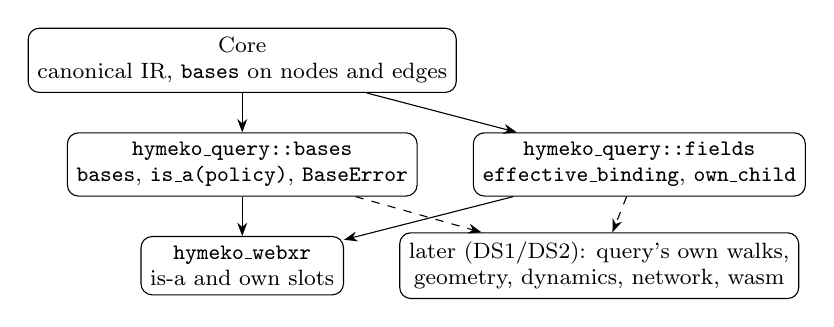
\begin{tikzpicture}[node distance=5mm and 7mm,every node/.style={draw,rounded corners,align=center,font=\footnotesize},>={Stealth}]
\node (core) {Core\\canonical IR, \texttt{bases} on nodes and edges};
\node (bases) [below=of core] {\texttt{hymeko\_query::bases}\\\texttt{bases}, \texttt{is\_a(policy)}, \texttt{BaseError}};
\node (fields) [right=of bases] {\texttt{hymeko\_query::fields}\\\texttt{effective\_binding}, \texttt{own\_child}};
\node (webxr) [below=of bases] {\texttt{hymeko\_webxr}\\is-a and own slots};
\node (later) [right=of webxr] {later (DS1/DS2): query's own walks,\\geometry, dynamics, network, wasm};
\draw[->] (core)--(bases); \draw[->] (core)--(fields);
\draw[->] (bases)--(webxr); \draw[->] (fields)--(webxr);
\draw[->,dashed] (bases)--(later); \draw[->,dashed] (fields)--(later);
\end{tikzpicture}

\end{center}
\end{document}
